
\section{2D Unmanned Aircraft System}\label{sec:2d_sim}
\paragraph{}As it is mentioned earlier, the first approach to the problem was addressed in a cartesian 2-dimensional system. This implies only 1 degree of freedom in our system, being that the azimuth angle ($\theta$). The system is composed of two controllers, one for the UA and one for Ground Station, which have the goal to take the angle of their respective devices to the reference signal (optimal angle). In this section an algorithm to calculate the optimal angle for the 2D system will be introduced. Furthermore the implementation of the controllers will be explained.

\subsection*{Scenario}

\begin{figure}[h]
	\centering
	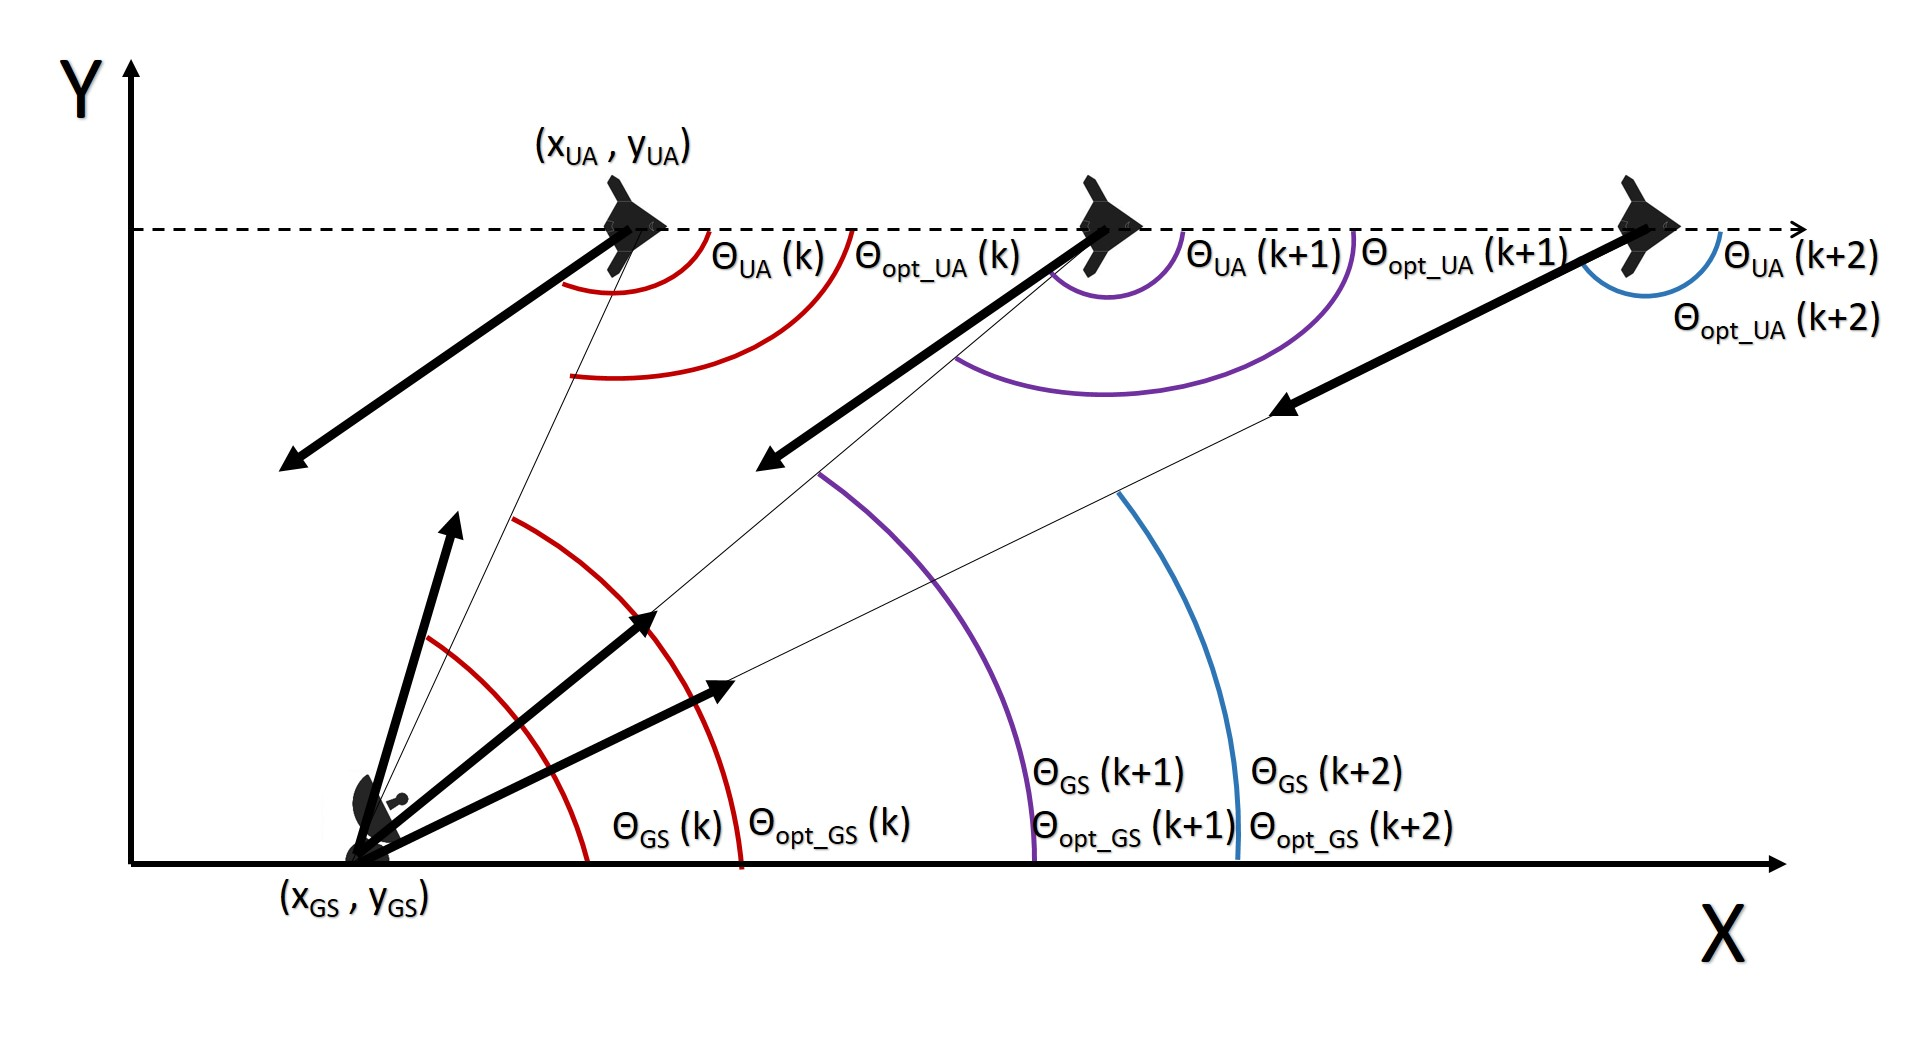
\includegraphics[scale=0.45]{figures/drone_gs_ex_1.jpg}
	\caption{GS-UA scenario example.}
	\label{fig:ua_gs}
\end{figure}

\paragraph{}In Figure \ref{fig:ua_gs} it is shown a scenario where the antennas of both GS and UA change after some periods of time. In the top part of the figure it is shown the angle of the drone ($\theta_{D}$) and the optimal angle ($\theta_{Dopt}$) that the antenna need to be driven to. In the lower part of the figure it is shown the angle of the GS ($\theta_{GS}$) and the optimal angle ($\theta_{GSopt}$) for it. 

As it is seen on the figure, at the starting time k the antenna on the UA ($\theta_{D} (k)$) is not pointing to the ground station, and therefore not equal to the optimal angle ($\theta_{Dopt}(k)$). The same goes with the $\theta_{GS}(k)$ and its reference $\theta_{GSopt}(k)$. As time passes, the controllers will drive the antenna angles to their reference, and therefore making them point at each other. 

\subsection*{System overview}
The following block diagram represents the system that simulates the scenario presented above:
\begin{figure}[H]
	\centering
	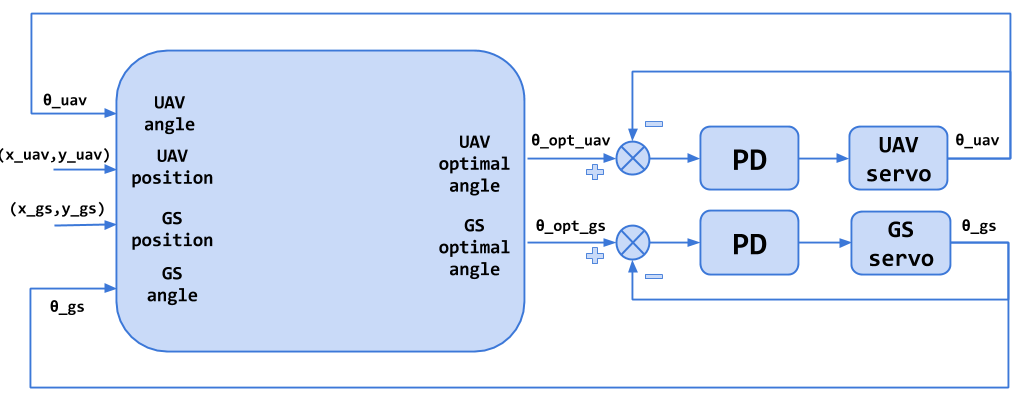
\includegraphics[scale=0.50]{figures/2d_system.png}
	\caption{2D Block diagram system.}
	\label{fig:2d_system}
\end{figure}

\paragraph{} The first block of the system is the one in charge of making all the geometric calculations derived in Section \ref{sec:optimal_angle} in order to calculate the reference. The input parameters to do this function are, in the simple 2D scenario, only the position of both UA and GS.

\paragraph{} After the reference is calculated, the usual "feedback control" scenario is shown, where the reference is compared with the feedback output signal and then inputed into the designed controller (Chapter \ref{ch:controller}) and the model of Moving Angle System (MAS, Chapter \ref{sec:moving_angle_system}), which will give the angle of the antenna as the output.

% \subsection{Simulations}
% To verify that the 2D simulations work, some simulations are made. In the first simulation the UA is simulated by starting in (0,50) and going to (100,50), which means that the aircraft is only moving in the x-axis. The simulation is shown in figure \ref{fig:gs_angle_vs_optimal} where the top one is showing the UA angle versus the optimal angle and the bottom one is showing the GS angle versus the optimal one. 

% \begin{figure}[h]
% 	\centering
% 	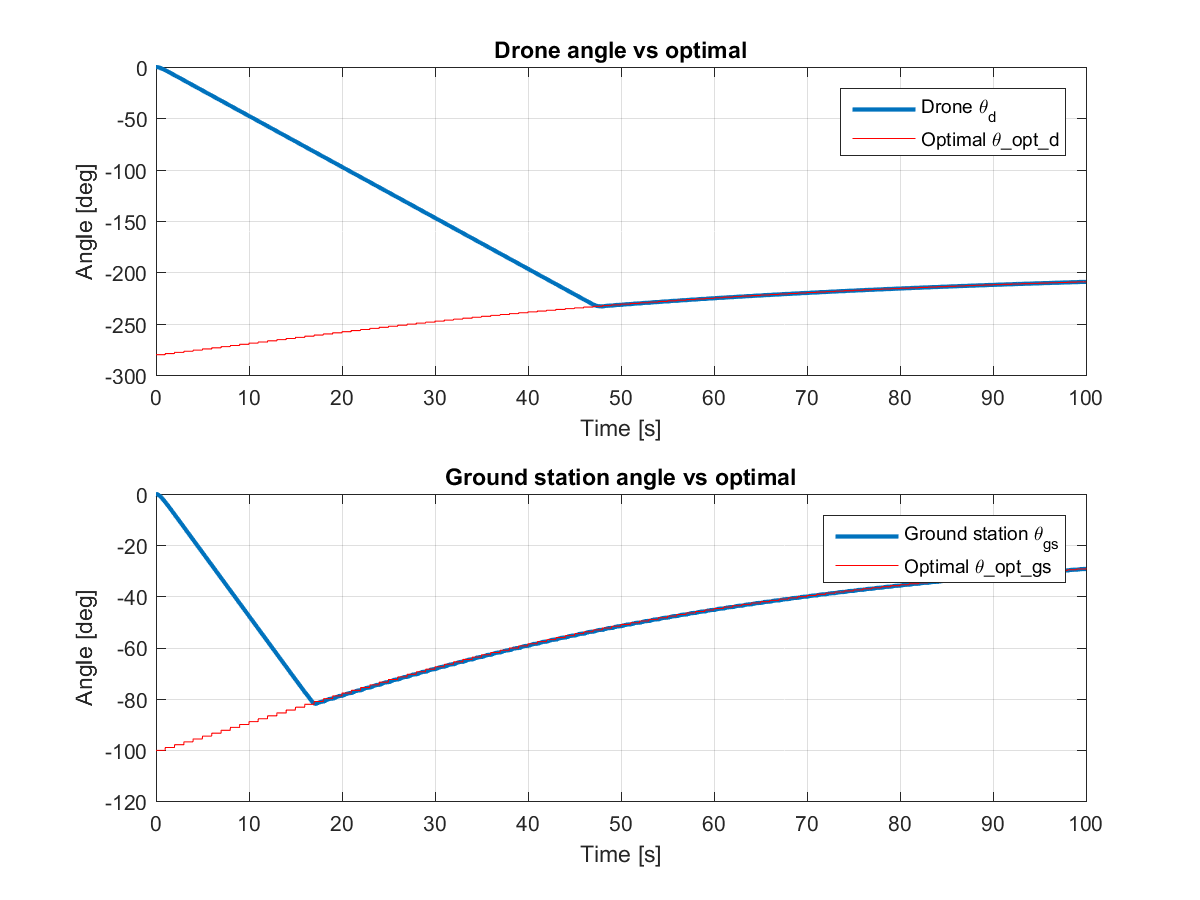
\includegraphics[scale=0.6]{figures/gs_angle_vs_optimal.png}
% 	\caption{GS angle vs optimal}
% 	\label{fig:gs_angle_vs_optimal}
% \end{figure}

% In this plot the angle is shown in degree to make it easier to understand. The blue line in both plots is respectively the UA and the GS antenna angle. They both start in 0 degree and have no initial starting point. Here it takes about 46 seconds for the UA's antenna to be at the optimal angle and in the other case it takes about 17 seconds for the GS antenna to turn to the optimal angle. But when they reached their optimal angle, the controller holds the antennas to the optimal angle. 
% \newpage
